\documentclass[tikz, preview]{standalone}
\usepackage{amsfonts, amsthm, amssymb, amsmath, stmaryrd, etoolbox}
\usepackage{tikz}
\usetikzlibrary{matrix,arrows}
\begin{document}
%%%%%%%%%%%%%%%%%	
%%%%%%%%%%%%%%%%%
\[
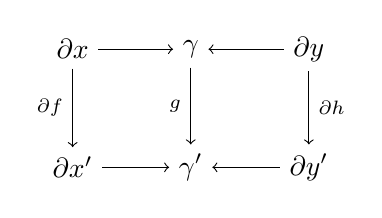
\begin{tikzpicture}
%	\draw [help lines, step=0.2, color=blue!10] (-5,-5) grid (5,5); % grid
	\node (1) at (-1.5,1.5) {$ \partial x $};
	\node (2) at (0,1.5) {$ \gamma $};
	\node (3) at (1.5,1.5) {$ \partial y $};
	\node (4) at (-1.5,0) {$ \partial x' $};
	\node (5) at (0,0) {$ \gamma' $};
	\node (6) at (1.5,0) {$ \partial y' $};
	\draw [->] (1) to (2);
	\draw [->] (3) to (2);
	\draw [->] (4) to (5);
	\draw [->] (6) to (5);
	\draw [->] (1) to node [left] {\scriptsize $ \partial f $} (4);
	\draw [->] (2) to node [left] {\scriptsize $ g $} (5);
	\draw [->] (3) to node [right] {\scriptsize $ \partial h $} (6);
\end{tikzpicture}
\]
%%%%%%%%%%%%%%%%%
%%%%%%%%%%%%%%%%%
\end{document}
